% Draft. Compile with:
%   pdflatex main && bibtex main && pdflatex main && pdflatex main
% Figures are read from ../figures/, produced by ../experiments/make_figures.py.
\documentclass[11pt]{article}

\usepackage[margin=1in]{geometry}
\usepackage{amsmath,amssymb,amsthm}
\usepackage{graphicx}
\usepackage{booktabs}
\usepackage[round,authoryear]{natbib}
\usepackage[hidelinks]{hyperref}

\graphicspath{{../figures/}}

\newcommand{\E}{\mathbb{E}}
\newcommand{\KL}{\mathrm{KL}}
\newcommand{\F}{\mathcal{F}}
\newcommand{\G}{\mathcal{G}}

\newtheorem{theorem}{Theorem}
\newtheorem{proposition}{Proposition}
\newtheorem{corollary}{Corollary}
\theoremstyle{remark}
\newtheorem{remark}{Remark}

\title{Supplement to ``Betting against the simulator:\\
Monte Carlo e-processes under adaptive actions''}

\author{Elena Bortolato\\ CUNEF Universidad}

\date{\today}

\renewcommand{\thesection}{S\arabic{section}}
\renewcommand{\thetable}{S\arabic{table}}
\renewcommand{\thefigure}{S\arabic{figure}}

\begin{document}
\maketitle

This supplement contains three analyses referred to in the main text, in
Section~S4 additional results for Sections~5 and~6, and in Section~S5 the
classical forms of the predictive factorisation used in Section~4. Theorem,
section, equation and table numbers without an S refer to the main text.

\section{Monitoring one patient under closed-loop control}\label{sec:t1d-patient}

This section uses the simulator of Section~6.1 of the main
text, with one additional source of randomness: unannounced snacks of between
5 and 25~g, with probability 0.01 per five-minute interval.

\paragraph{The data.} The ``real'' patient is \texttt{simglucose}'s
\texttt{adult\#001}, followed for 48 hours with three meals a day at jittered
times. It is treated by basal--bolus therapy with feedback, using the
patient's own basal rate, carbohydrate ratio and correction factor. Every 30
minutes (an \emph{epoch}) the controller commits to a basal rate from the
current CGM reading:
\begin{itemize}
  \item basal is suspended below 80~mg/dL;
  \item a correction is added above 180~mg/dL;
  \item within the epoch, meal boluses follow the announced carbohydrates.
\end{itemize}
All dosing decisions therefore depend on the data. At hour 12 the patient may
change in one of three ways, chosen to mimic common clinical failures:
\begin{itemize}
  \item \textbf{Insulin resistance:} $V_{mx}$ and $k_{p3}$ fall by 30\%, as
        during an infection.
  \item \textbf{Sensor drift:} the CGM gain increases linearly from 1 to 1.15
        over the following 24 hours, a slow calibration failure.
  \item \textbf{Snacking:} unannounced snacks become six times as frequent.
\end{itemize}
In the null scenario the patient remains the twin throughout.

\paragraph{Monitoring.} At the start of each epoch the twin is
re-initialised at the patient's current state and run $M = 16$ times under the
committed dosing plan and the announced meals, producing 16 simulated 30-minute
CGM traces. A seventeenth, noise-free run gives the twin's prediction $g_t$.
Each trace is summarised relative to $g_t$ by:
\begin{itemize}
  \item its mean residual and its residual over the last five minutes;
  \item the change in residual between the first and the last ten minutes;
  \item two context variables: the predicted glucose level and the committed
        insulin rate.
\end{itemize}
The score is the BLR predictive of Section~4.3 on these
summaries, updated after every epoch.

Because the dosing plan is committed at the start of the epoch, the epoch's
action is $\G_t$-measurable, and Theorem~1 applies with each
epoch as one step. The 30-minute epoch is a design choice made for power. With
the twin re-initialised every five minutes, a 30\% loss of insulin sensitivity
moves the one-step prediction by only about 0.1~mg/dL, against a CGM noise of
several mg/dL. Over 30 minutes the mean residual moves by about 3~mg/dL,
against a spread of about 2~mg/dL between twin draws.

We compare four monitors:
\begin{itemize}
  \item the BLR predictive score;
  \item a fixed score equal to the mean residual of the epoch, with no
        learning;
  \item the same BLR monitor with the twin run under the \emph{open-loop}
        plan (basal and meal boluses, without suspension or correction), that
        is, not conditioned on the action actually taken;
  \item a $t$-test of standardised epoch residuals, recomputed after every
        epoch.
\end{itemize}

\begin{figure}[t]
\centering
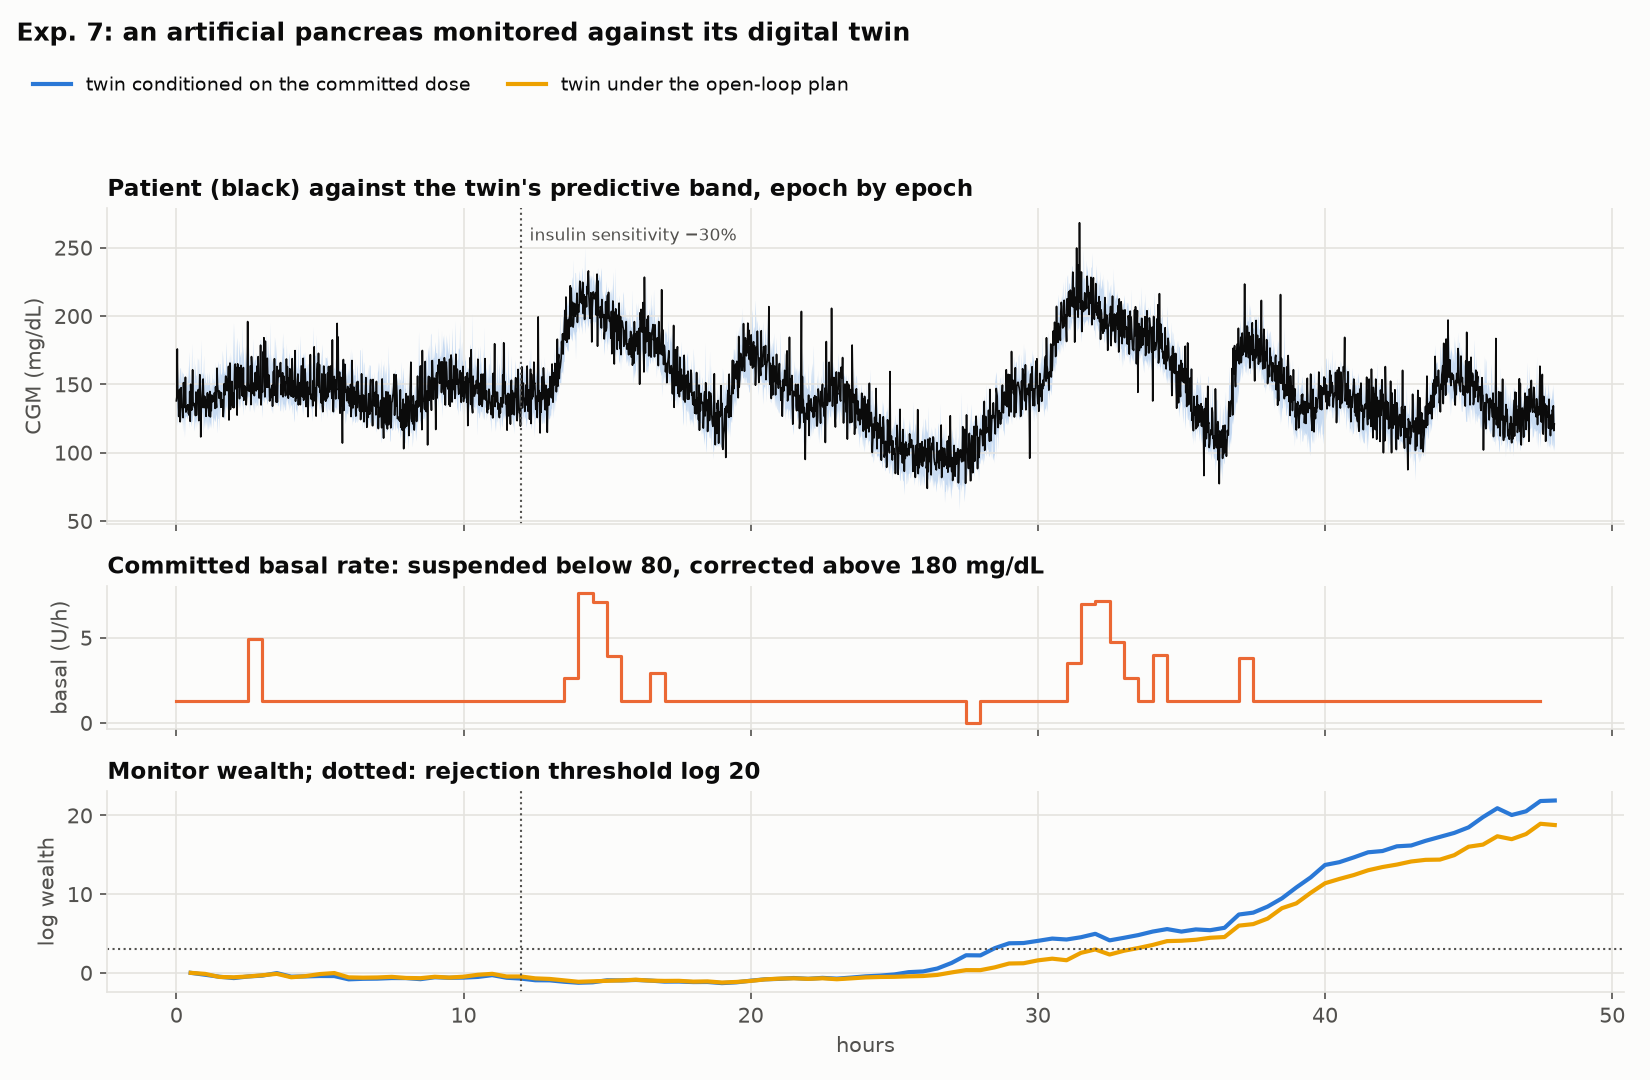
\includegraphics[width=\textwidth]{exp7_artificial_pancreas.png}
\caption{One monitored patient whose insulin sensitivity falls by 30\% at
hour 12. Top: CGM readings (black) and the twin's 5--95\% predictive band,
recomputed at the start of every 30-minute epoch from the patient's current
state and the committed dose. Middle: the committed basal rate, suspended below
80~mg/dL and corrected above 180~mg/dL. Bottom: log wealth of the monitor, with
the rejection threshold $\log 20$.}
\label{fig:application}
\end{figure}

\paragraph{Results.} Table~\ref{tab:t1d} summarises 200 null runs and 80 runs
of each failure scenario.

\begin{table}[t]
\centering
\caption{Artificial pancreas against its digital twin (48 hours; changes at
hour 12). Null: share of runs with an alarm. Failure scenarios: share
detected within the 36 hours after the change, and median delay in hours.
For the recomputed $t$-test, 22.5\% of runs in every scenario had already
raised a (false) alarm before the change.}
\label{tab:t1d}
\begin{tabular}{lrrrr}
\toprule
monitor & null & insulin resistance & sensor drift & snacking \\
\midrule
MC e-process, BLR score & 0.010 & 1.00, 10.5 h & 1.00, 10.0 h & 0.14, 27 h \\
MC e-process, fixed residual score & 0.030 & 1.00, 9.0 h & 1.00, 8.8 h & 0.30, 23 h \\
twin under the open-loop plan & 0.000 & 1.00, 9.8 h & 1.00, 10.0 h & 0.16, 30 h \\
$t$-test, recomputed every epoch & 0.350 & 0.78, 7.5 h & 0.78, 8.5 h & 0.23, 20 h \\
\bottomrule
\end{tabular}
\end{table}

\begin{itemize}
  \item \textbf{Validity with a black-box simulator.} The Monte Carlo
        e-process keeps false alarms at 1\% over 48 hours, with a simulator
        whose outcome law has no tractable density. The recomputed $t$-test
        raises false alarms in 35\% of runs, and in 22.5\% of runs before any
        change has occurred.
  \item \textbf{Physiological and sensor failures are detected within a
        day.} A 30\% loss of insulin sensitivity is detected in every run,
        after a median of 10.5 hours; a slow calibration drift after 10 hours
        (Figure~\ref{fig:application}).
  \item \textbf{Sparse disturbances are hard.} More frequent unannounced
        snacks are detected in only 14\% of runs within 36 hours: they appear
        as occasional upward jumps, which the smooth learned score captures
        poorly. The fixed mean-residual score does better (30\%); a score
        designed for jumps would do better still.
  \item \textbf{When conditioning on the action does not matter.} Here the
        twin run under the open-loop plan is also valid (no false alarms). For
        this patient, suspension and correction are triggered rarely, and when
        they are, they barely change the distribution of the next 30 minutes.
        Proposition~2 shows where the danger lies: ignoring
        the action inflates the bet when the actions taken change the law of
        the outcome, $\chi^2(P_a\|\bar P) > 0$, and it is nearly harmless when
        they do not. The bandit
        (Section~5.2) and the language-model audit
        (Section~5.6) are cases where it does.
\end{itemize}

\paragraph{Limitations.} The patient is itself
simulated, so this is a realistic benchmark rather than a clinical
validation. The twin is re-initialised at the patient's true physiological
state, which is observable in silico but must be estimated in practice. With
an estimated state, the null law of the next epoch is the twin's filtering
predictive distribution; sampling from it approximately breaks exact
exchangeability, and the guarantees of \citet{barber2026montecarlo} for
approximately exchangeable samples are the natural tool. Real CGM and insulin
records, such as those collected in closed-loop trials, would be the next
step.

\section{A single-stage response-adaptive trial}\label{sec:trial3}

This is a simpler version of the trial of Section~6 of the main
text, with three arms, one stage, one day per participant and Thompson-sampling
allocation (Experiment~10 in the repository).

\paragraph{The trial.} The same simulator is used to design clinical trials of
dosing strategies: arms are compared in silico before the trial, and the
simulator's predictions justify the design and sample size. We consider a
three-arm trial of insulin-dosing strategies, each run by the pump in closed
loop:
\begin{itemize}
  \item \textbf{A, standard:} carbohydrate bolus, correction to 140~mg/dL above
        150, basal suspended below 80;
  \item \textbf{B, aggressive:} bolus $\times 1.5$, correction to 100, suspend
        below 60;
  \item \textbf{C, conservative:} bolus $\times 0.8$, correction to 160, suspend
        below 90.
\end{itemize}
Participants enter one at a time; each is one of the ten adult virtual
patients, drawn at random, and spends one in-clinic day (06:00--18:00, with a
standardised breakfast of 50~g at 07:00 and lunch of 70~g at 12:30) under the
assigned arm. The primary outcome is time in range (70--180~mg/dL).
Allocation is response-adaptive, as in Bayesian adaptive trials: after a
burn-in of 15 participants in permuted blocks, each participant is assigned by
Thompson sampling on the arms' mean time in range, with allocation
probabilities floored at 0.1. The trial enrols 120 participants.

\paragraph{The twin and the question.} The twin is the in-silico trial itself:
for each participant, the simulator with that participant's virtual-patient
parameters is run $M = 16$ times under the arm actually assigned and the same
meal protocol. The monitor asks whether the in-silico trial still predicts
what happens to the participants \emph{given the allocation the design has
made}. The score is the BLR predictive of Section~4.3 on six
summaries of the day relative to the twin's noise-free path (mean and standard
deviation of the residual, time below 70 and above 180 mg/dL, and the arm),
with interactions between the arm and the residual and time-below-range
features, so that the score can learn a discrepancy confined to one arm. We
compare it with the plug-in bet, a $t$-test of standardised time-in-range
residuals recomputed after every participant, and a \emph{pooled} twin that
simulates each participant under an arm drawn uniformly. The pooled twin is the
pre-trial in-silico prediction, which ignores the allocation.

\paragraph{Which arm?} A single alarm says that the twin fails somewhere; a
trial team needs to know under which arm. We run one e-process per arm, each
with its own BLR score, which bets only on the participants assigned to that
arm and has factor one otherwise. Whether a participant goes to arm $k$ is
decided before the outcome, so by Theorem~1 each is a test
martingale for $H_{0,k}$: ``the twin is correct under arm $k$'', whatever the
allocation. Each arm's e-value is its wealth at the end of the trial, or when
it first reaches $K/\alpha$ with $K = 3$ (a bounded stopping time), and e-BH
\citep{wang2022false} is applied across the arms. This is the bandit
multiple-testing construction of \citet{xu2021unified}, with the twin as the
null; e-BH controls the false discovery rate under arbitrary dependence
between the arms, which the shared allocation creates.

\paragraph{Scenarios.} Under the null, participants are the simulator. Two
departures are considered:
\begin{itemize}
  \item \textbf{Insulin resistance.} Insulin sensitivity is 25\% lower than in
        the virtual cohort, in every arm.
  \item \textbf{Rescue carbohydrates.} Participants self-treat hypoglycaemia,
        taking 15~g of carbohydrate when the CGM reads below 70~mg/dL, at most
        every 30 minutes. The simulator omits this behaviour. Its effect
        depends on the arm: it matters under the aggressive arm, which causes
        most lows. In the twin, arm B spends 10\% of the day below 70~mg/dL; in
        the participants it spends 2\% and has the best time in range.
\end{itemize}

\begin{table}[t]
\centering
\caption{A response-adaptive three-arm trial of 120 participants checked
against its in-silico twin (200 replications per scenario). Rejection rate by
the end of the trial and, in brackets, the median number of participants
before the first alarm. Allocation: share of participants assigned to the
aggressive arm B after the burn-in. The last block reports which arms e-BH
flags at $\alpha = 0.05$ at the end of the trial.}
\label{tab:trial3}
\begin{tabular}{lrrr}
\toprule
monitor & null & insulin resistance & rescue carbohydrates \\
\midrule
MC e-process, twin under the assigned arm & 0.025 & 1.00 (5) & 1.00 (27) \\
plug-in bet & 0.095 & 1.00 (6) & 1.00 (33) \\
pooled twin (ignores the allocation) & 0.415 & 1.00 (11) & 1.00 (38) \\
$t$-test, recomputed & 0.390 & 1.00 (9) & 0.995 (23) \\
\midrule
share allocated to arm B & 0.36 & 0.83 & 0.74 \\
time in range under B: participants / twin & 0.87 / 0.87 & 0.89 / 0.87 & 0.94 / 0.87 \\
\midrule
\multicolumn{4}{l}{\emph{per-arm e-processes and e-BH: share of trials in which each arm is flagged}} \\
arm A (standard) & 0.000 & 1.00 & 0.005 \\
arm B (aggressive) & 0.015 & 1.00 & 1.00 \\
arm C (conservative) & 0.000 & 1.00 & 0.005 \\
rescue events per trial on A / B / C & -- & -- & 3.7 / 155 / 0.2 \\
\bottomrule
\end{tabular}
\end{table}

\paragraph{Results.} Table~\ref{tab:trial3} summarises 200 replications of
each scenario.
\begin{itemize}
  \item \textbf{Only the conditioned monitor is valid.} Its false-alarm rate is
        2.5\%. The pooled twin raises a false alarm in 42\% of trials: once the
        allocation concentrates on arms A and B, the participants are no longer
        a sample from the pre-trial mixture over arms, exactly as
        Proposition~2 predicts. The recomputed $t$-test
        raises false alarms in 39\% of trials, and the plug-in bet in 9.5\%.
  \item \textbf{Insulin resistance} is detected in every trial after a median
        of five participants. The allocation adapts to it: resistant
        participants do best on the aggressive arm, which receives 83\% of
        them.
  \item \textbf{Rescue carbohydrates} change mainly arm B, and the monitor
        detects them in every trial after a median of 27 participants. The
        design reacts to the same discrepancy: arm B looks better than the
        twin predicted, so it receives 74\% of the participants instead of
        36\% under the null. The twin that justified the design is therefore
        wrong precisely on the arm the design ends up favouring, and it is
        wrong in a direction a sponsor would not look for, since the
        participants do better than predicted. Detection is slower than for
        resistance because the departure is confined to one arm and to the
        hours around lows.
  \item \textbf{e-BH names the arm.} Under the null, e-BH flags some arm in
        1.5\% of trials. Under insulin resistance, which affects every arm, it
        flags all three arms in every trial, including the conservative arm,
        which receives only about 14 participants. Under rescue carbohydrates
        it flags arm B in every trial and arms A and C in 0.5\% each, a false
        discovery proportion of 0.5\% on average if A and C are counted as
        nulls. Arm A is in fact affected weakly (3.7 rescue events per trial,
        against 155 under B), too weakly to be detected: e-BH points to the
        arm on which the twin materially fails.
\end{itemize}
The pooled twin and the $t$-test also reject under both departures, but they
reject under the null as well, so their alarms carry no evidence. The trial
illustrates the setting of Theorem~1 with clinical actions: the
allocation is chosen from the outcomes, the null is only available as a
simulator, and a monitor that ignores the allocation is invalid.

%======================================================================
\section{Comparison with the Besag--Clifford e-process}\label{sec:exp-bc}

On the drift task the null is i.i.d., so the Besag--Clifford e-process of
\citet{dombowsky2026besag} applies directly. We compare statistics and betting
strategies on identical data and identical simulator draws ($M = 16$).
\begin{itemize}
  \item \textbf{Statistics:}
        \begin{itemize}
          \item the likelihood ratio recommended by their Theorem~1, which
                requires both densities and the true alternative (an oracle);
          \item their plug-in approach for a composite alternative (their
                Sections~3.2 and~6.3), with the maximum-likelihood curvature
                computed from past data only, which requires the density of the
                parametric family;
          \item our BLR predictive score, which requires only samples from the
                simulator.
        \end{itemize}
  \item \textbf{Betting:} all-in ($\lambda = 1$, their likelihood-ratio
        process), aGRAPA \citep{waudbysmith2024estimating}, and the mixture
        (3).
\end{itemize}

\begin{table}[t]
\centering
\caption{Besag--Clifford e-process with different statistics and betting
strategies on the drift task (400 replications). Entries: false-alarm rate,
power, median stopping time.}
\label{tab:bc}
\begin{tabular}{llrrr}
\toprule
statistic (requires) & betting & false alarms & power & median stop \\
\midrule
likelihood ratio (both densities, true alternative) & all-in & 0.045 & 1.000 & 36 \\
 & aGRAPA & 0.010 & 1.000 & 66 \\
 & mixture & 0.018 & 1.000 & 48 \\
plug-in MLE (density of the parametric family) & all-in & 0.022 & 1.000 & 58 \\
 & aGRAPA & 0.010 & 1.000 & 86 \\
 & mixture & 0.010 & 1.000 & 68 \\
BLR predictive (simulator samples only) & all-in & 0.028 & 0.405 & -- \\
 & aGRAPA & 0.005 & 0.938 & 289 \\
 & mixture & 0.018 & 0.983 & 209 \\
\bottomrule
\end{tabular}
\end{table}

Table~\ref{tab:bc} quantifies the price of not knowing the model.
\begin{itemize}
  \item When the likelihood ratio is available, the Monte Carlo normalisation
        costs almost nothing: the median stopping time with $M = 16$ is 36,
        against 35 for the exact oracle (Table~1), as their
        Theorem~1 predicts.
  \item Knowing the parametric family of the drift is worth a factor of about
        3.5 in stopping time over learning it from samples (58 against 209).
  \item With a learned score, all-in betting fails: early misspecified bets
        drive the wealth towards zero, and power falls to 0.41. The mixture over
        $\lambda$ is the right strategy for learned scores, and it is faster
        than aGRAPA (209 against 289).
\end{itemize}
The two approaches are therefore complementary. When the null density is
known up to a constant and the alternative is parametric, the Besag--Clifford
statistic of \citet{dombowsky2026besag} should be used. When the simulator is
a black box, only a learned score is available, and the results of
Sections~3--4.1 govern its power. In adaptive
designs their i.i.d.\ formulation does not apply: simulating without
conditioning on the action rejects a true null in every run
(Table~2).

%======================================================================

\section{Additional results for Sections 5 and 6}\label{sec:more}

This section collects material moved out of the main text: the rejection
curves of the drift experiment, all variants of the update rules, the regret
check of Theorem~3, the growth rate as a function of the budget, the trial
with each learner, and all variants of the comparison with concurrent methods,
with the details of the alternatives outside SLICE's family.

\subsection{Drift experiment: rejection curves}

\begin{figure}[t]
\centering
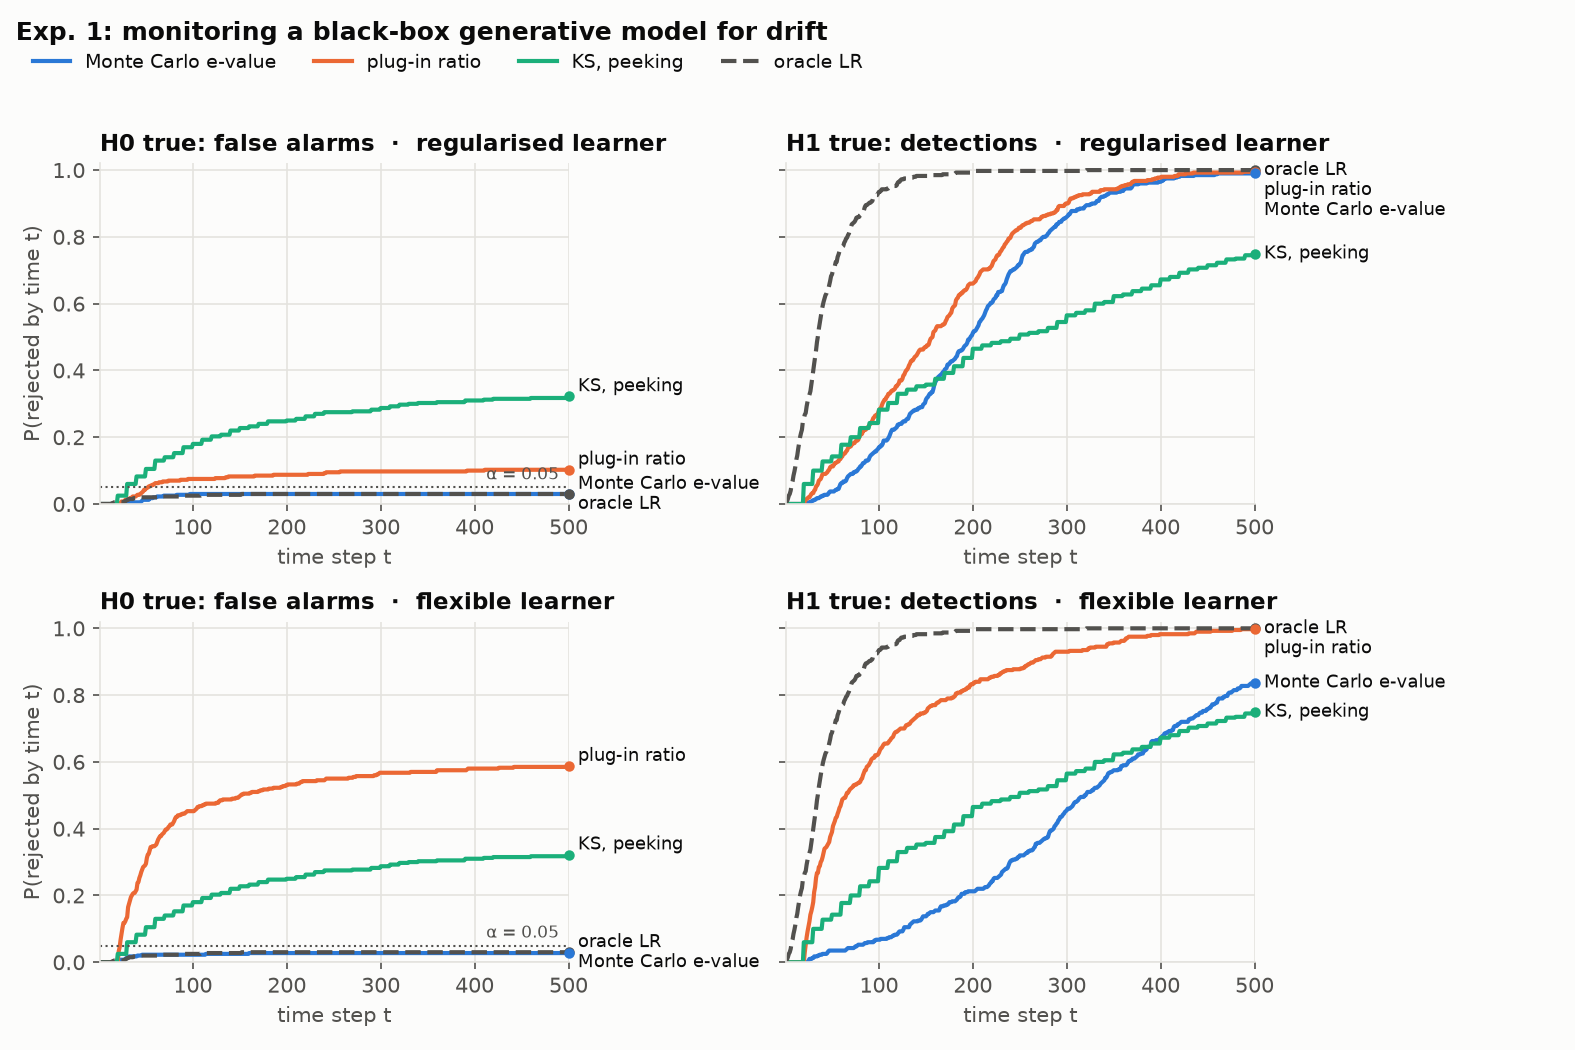
\includegraphics[width=\textwidth]{exp1_generative_drift.png}
\caption{Probability of having rejected by time $t$ in the generative-drift
experiment. Left: the null is true (false alarms). Right: the model has
drifted (detections). The dotted line is $\alpha = 0.05$.}
\label{fig:drift}
\end{figure}

\subsection{Update rules: all variants}


Table~\ref{tab:blr-full} compares, on the drift task and the bandit with identical
data, the refitted point estimate with the online Bayesian learning rule of
Section~4.3 of the main text, updated at every step with no burn-in. With the
logistic loss, the probability-scale predictive $\kappa\bar\eta$ beats the posterior
mean in every setting and makes the method insensitive to the flexibility of
the features: with degree-6 features power rises from 0.84 to 0.97 and the
median stopping time falls from 320 to 214, close to the degree-4 value, and in
the bandit it is the fastest score (38 against 49 steps). The ratio-scale
predictive $\mu + v/2$ is the worst score in every setting, with power 0.74--0.81
in the drift task, as its uncertainty premium over-bets where the Gaussian
approximation is least reliable. On the simulation likelihood, the
posterior-predictive bet beats the plug-in bet at the posterior mean (223
against 265 steps), as Proposition~4 suggests, and with a prior
variance of 0.03 it comes within 7\% of the logistic learner (223 against 209
steps with degree 4, 222 against 214 with degree 6); with the default prior
variance of one it needs 290 steps. The two learners fail in opposite
directions: the logistic learner's bets are aggressive (in steps 100--250 the
factors have mean 1.18 and standard deviation 1.15, and the best betting
fraction is 0.5), and the mixture over $\lambda$ tempers them, whereas the
simulation-likelihood bets are cautious (mean 1.08, standard deviation 0.62,
best fraction 0.75), and a fraction below one cannot amplify a cautious bet.
False alarms stay between 1.0\% and 3.3\% for every score; using the logistic
posterior odds directly as the bet gives between 14\% and 74\% false alarms.

The predictive-first updates (equation (9) of the main text) are valid in every setting and
slower than their Gaussian counterparts on the drift task: 234--277 steps with
degree-4 features, against 209--223, and with the flexible degree-6 features the
plug-in and resampled predictives lose much of their power (0.65 and 0.64,
against 0.97). On the bandit they are on par (41--57 steps, against 38--51).
Predictive resampling helps slightly on the drift task (234 against 243 steps
on the simulation likelihood), and the simulation likelihood is the better
loss for predictive-first updates, as it is for the posterior mixture. The
Gaussian route's advantage comes from its shrinkage: the posterior covariance
damps early bets for as long as the posterior is wide, whereas truncated
predictive resampling quickly concentrates around the current predictive.
The Bayesian-bootstrap forest is valid as well (4.5\% false alarms on the drift
task over 400 null runs, 2.0\% on the bandit), and it is the slowest learner on
these problems: a power of 0.61 within 500 steps on the drift, where the
discrepancy is a smooth change of curvature that a polynomial score represents
directly and trees approximate by axis-aligned steps, and a median of 63 steps
on the bandit. The mixture over trees and the forest's mean log-odds perform
alike. The forest is built as follows. The exchangeable units are the
monitoring steps, each contributing its real outcome (label one, weight one)
and its $M$ simulations (label zero, weight $1/M$), and each of $N = 16$ trees
of depth at most 6 is fitted to the past steps with its own
$\mathrm{Dirichlet}(1, \ldots, 1)$ weights, so that the forest is a sample from
the martingale posterior of the empirical predictive, the Bayesian bootstrap.
A leaf's score is its log-odds under a $\mathrm{Beta}(a, a)$ prior on its
weighted class counts, $\log\{(w_1 + a)/(w_0 + a)\}$ with $a = 3$, so that
leaves supported by little data bet little, and the bet is the mixture
$N^{-1}\sum_b E_t(\mathrm{tree}_b)$; each tree is fitted on the past only, so
the mixture is exactly fair.

\begin{table}[t]
\centering
\caption{Update rules, MC e-process throughout (400 replications). BLR: online
Bayesian learning rule on the logistic loss (probability-scale predictive
$\kappa\bar\eta$, ratio-scale $\bar\eta+v/2$, or posterior mean $\bar\eta$) or on the
simulation likelihood (posterior-predictive mixture bet, or plug-in at the
posterior mean; prior variance in brackets); predictive update: the
classifier's predictive updated directly by equation (9) of the main text, betting with the
current predictive (plug-in) or averaging over predictive-resampling paths;
Bayesian-bootstrap forest: trees fitted with Dirichlet weights (the martingale
posterior of the empirical predictive) on the raw outcomes, refitted every 25
steps from step 20.}
\label{tab:blr-full}
\begin{tabular}{llrrr}
\toprule
task & score & false alarms & power & median stop \\
\midrule
drift, degree 4 & refitted point estimate & 0.030 & 0.990 & 198 \\
 & BLR logistic, posterior mean & 0.030 & 0.965 & 238 \\
 & BLR logistic, probability scale & 0.018 & 0.983 & 209 \\
 & BLR logistic, ratio scale & 0.015 & 0.810 & 340 \\
 & BLR simulation likelihood, mixture (1) & 0.025 & 0.820 & 291 \\
 & BLR simulation likelihood, mixture (0.03) & 0.013 & 0.968 & 223 \\
 & BLR simulation likelihood, mean (0.03) & 0.025 & 0.938 & 265 \\
 & predictive update, logistic, plug-in & 0.020 & 0.810 & 277 \\
 & predictive update, logistic, resampling & 0.022 & 0.802 & 266 \\
 & predictive update, simulation likelihood, plug-in & 0.018 & 0.895 & 243 \\
 & predictive update, simulation likelihood, resampling & 0.010 & 0.920 & 234 \\
 & Bayesian-bootstrap forest, mixture over trees & 0.045 & 0.605 & 420 \\
 & Bayesian-bootstrap forest, mean log-odds & 0.045 & 0.620 & 411 \\
drift, degree 6 & refitted point estimate & 0.028 & 0.838 & 320 \\
 & BLR logistic, posterior mean & 0.033 & 0.940 & 242 \\
 & BLR logistic, probability scale & 0.015 & 0.965 & 214 \\
 & BLR logistic, ratio scale & 0.013 & 0.738 & 364 \\
 & BLR simulation likelihood, mixture (0.03) & 0.018 & 0.915 & 222 \\
 & predictive update, logistic, plug-in & 0.033 & 0.650 & 353 \\
 & predictive update, logistic, resampling & 0.025 & 0.643 & 363 \\
bandit & refitted point estimate & 0.028 & 1.000 & 49 \\
 & BLR logistic, posterior mean & 0.025 & 1.000 & 51 \\
 & BLR logistic, probability scale & 0.030 & 1.000 & 38 \\
 & BLR logistic, ratio scale & 0.025 & 0.995 & 106 \\
 & predictive update, logistic, plug-in & 0.025 & 1.000 & 41 \\
 & predictive update, logistic, resampling & 0.025 & 1.000 & 42 \\
 & predictive update, simulation likelihood, plug-in & 0.010 & 1.000 & 54 \\
 & predictive update, simulation likelihood, resampling & 0.013 & 1.000 & 57 \\
 & Bayesian-bootstrap forest, mixture over trees & 0.020 & 0.998 & 63 \\
\bottomrule
\end{tabular}
\end{table}


\subsection{Regret of the posterior-predictive e-process}

The set-up is given in the next subsection. Table~\ref{tab:regret}
reports the largest regret over the 12 paths of each scenario.

\begin{table}[t]
\centering
\caption{Regret of the exact posterior-predictive e-process against the best
score in hindsight, $\sup_\theta \log L_t(\theta) - \log \bar W_t$ (maximum
over 12 paths), and the bound of Theorem~3(ii). Slope: increase
of the mean regret per unit of $\log t$ between $t = 100$ and $t = 2000$.}
\label{tab:regret}
\begin{tabular}{lrrrrrrr}
\toprule
 & \multicolumn{5}{c}{maximum regret at $t =$} & & \\
scenario & 10 & 100 & 300 & 1000 & 2000 & slope & $\log \bar W_{2000}$ \\
\midrule
null & 1.9 & 4.1 & 5.1 & 6.3 & 7.0 & 1.02 & $-5.6$ \\
mean shift & 2.6 & 4.0 & 5.0 & 6.2 & 6.9 & 1.02 & 228 \\
scale change & 2.2 & 4.5 & 5.6 & 6.8 & 7.5 & 1.01 & 257 \\
drift at $t = 500$ & 1.9 & 4.1 & 5.1 & 6.5 & 7.3 & 1.10 & 236 \\
\midrule
bound, $d\log t + d\log(4eGD/d)$ & 10.9 & 15.5 & 17.7 & 20.1 & 21.5 & & \\
\bottomrule
\end{tabular}
\end{table}

\subsection{Growth rate and budget}

On the drift task with the regularised learner (200 replications), false
alarms stay between 1.5\% and 3.5\% at every budget, and the median stopping
time is 371 steps at $M = 1$ against 207 at $M = 64$, a factor 1.8 against the
factor 2 of Theorem~2(iv); for larger $M$ the ratios are smaller, as part of
the stopping time is spent learning the score. With $P = \mathcal N(0,1)$,
$Q = \mathcal N(\delta, 1)$ and $T(x) = e^{\theta x}$, for which
$\tilde T = \mathcal N(\theta, 1)$, $g_\infty = \theta\delta - \theta^2/2$ and
$\rho = e^{\theta\delta}$, the efficiency $g_M/g_\infty$ for $\delta = 0.25$ is
0.48, 0.66, 0.80, 0.89 and 0.93 at $M = 1, 2, 4, 8, 16$, against
$M/(M+1) = 0.50, 0.67, 0.80, 0.89, 0.94$. With $\theta = 2\delta$ and
$\delta = 1$, where $g_\infty = 0$, the growth rate rises to 0.18 at $M = 4$ and
falls towards zero as $M$ grows: a finite budget tempers an overconfident
score. The regret check of Theorem~3 uses the bounded features
$\phi(x) = (\mathrm{clip}(x, \pm 3), \mathrm{clip}(x^2 - 1, \pm 3))/3$ ($d = 2$,
$G = \sqrt 2$), a uniform prior on the disc of radius $D = 3$ and
$P = \mathcal N(0,1)$; the mixture is computed exactly on a grid of 31\,000
points and the hindsight optimum by convex optimisation, for 12 paths of each
scenario. Under the null the log wealth decreases, and under the alternatives
the monitor keeps pace with the best fixed score chosen in hindsight,
including after the change point, where that score is itself a compromise
between the two regimes.

\subsection{The trial with each learner}

Table~\ref{tab:trial-learners} compares all learners. The four predictive-first
learners of Section~4.3 of the main text are valid as well, with false alarms in 1--5\%
of trials while the stateless twin raises them in 81--98\%; they detect snacking
in 99\% of trials after a median of 42--51 participant-days, and e-BH flags D in
99\% of trials and B in 37--62\%, with A, C and E flagged in at most 2\%.
The Bayesian-bootstrap forest, refitted every ten participant-days from the
fifth, is valid (2\% false alarms) and the slowest to detect (a median of 59
participant-days), and e-BH flags B in 31\% of trials; refitted every 25 days
from the twentieth, as in the simulation studies, it flags B in only 3\%,
because an arm dropped at the first interim analysis leaves its own forest
too few days to be fitted before the arm stops accruing data.

\begin{table}[t]
\centering
\caption{The MAMS trial with each learner (100 replications per scenario).
Null: false-alarm rate of the monitor and of the stateless twin with the same
learner. Snacking: detection rate, median participant-days to the first alarm,
and the share of trials in which e-BH flags arms D and B.}
\label{tab:trial-learners}
\begin{tabular}{lrrrrr}
\toprule
 & \multicolumn{2}{c}{null} & \multicolumn{3}{c}{defensive snacking} \\
learner & monitor & stateless & detected (days) & e-BH D & e-BH B \\
\midrule
Gaussian BLR, logistic & 0.02 & 0.95 & 0.99 (32) & 0.99 & 0.64 \\
Gaussian BLR, simulation likelihood & 0.02 & 0.98 & 0.99 (51) & 0.99 & 0.39 \\
predictive, logistic, plug-in & 0.05 & 0.87 & 0.99 (42) & 0.99 & 0.62 \\
predictive, logistic, resampling & 0.04 & 0.81 & 0.99 (47) & 0.99 & 0.47 \\
predictive, simulation likelihood, plug-in & 0.04 & 0.98 & 0.99 (49) & 0.99 & 0.38 \\
predictive, simulation likelihood, resampling & 0.01 & 0.97 & 0.99 (51) & 0.99 & 0.37 \\
Bayesian-bootstrap forest & 0.02 & 0.98 & 0.99 (59) & 0.98 & 0.31 \\
\bottomrule
\end{tabular}
\end{table}

\subsection{Comparison with concurrent methods: all variants}

Table~\ref{tab:concurrent-full} reports every score of Section~5.5 of the main
text, including the refitted score with a weak penalty (prior variance 1
instead of 0.03), the score fitted in advance on a wrong guess of the
alternative (curvature 0.2 instead of 0.8), and SLICE with the exact
parametric ratio instead of the network, which is its best case. The
refitted score maximises the penalised growth by damped Newton steps with a
backtracking line search, every ten steps from step 20. SLICE's network is a
multilayer perceptron with three hidden layers of 128 units, trained by neural
ratio estimation (joint against shuffled pairs; SLICE uses the contrastive
NRE-C objective) on $2 \times 10^5$ pairs from a uniform prior over the
family, $b \in [0, 1.5]$ for the drift and a shift in $[-1, 1]$ for the bandit;
the parameter is estimated by maximum likelihood (drift) or by the arm's mean
(bandit) from past real data. Times are wall-clock seconds for 800 replications
on four cores; the simulations are cheap here, so they measure mostly the cost
of the score.

\begin{table}[h]
\centering
\caption{All scores of the comparison with concurrent methods (400
replications per scenario). Rate: share of runs that reject; median: median
stopping time under the alternative.}
\label{tab:concurrent-full}
\small
\begin{tabular}{llrrrr}
\toprule
scenario & score & false alarms & power & median & time (s) \\
\midrule
drift, in family & ours, BLR logistic & 0.018 & 0.983 & 209 & 63 \\
 & ours, simulation likelihood & 0.013 & 0.968 & 223 & 59 \\
 & F\&B refitted, penalty 0.03 & 0.020 & 0.988 & 200 & 200 \\
 & F\&B refitted, penalty 1 & 0.033 & 0.995 & 192 & 224 \\
 & F\&B fitted in advance, true alternative & 0.025 & 1.000 & 61 & -- \\
 & F\&B fitted in advance, wrong guess & 0.028 & 0.000 & -- & -- \\
 & SLICE, exact ratio & 0.007 & 1.000 & 75 & -- \\
 & SLICE, neural ratio & 0.007 & 1.000 & 71 & 91 \\
drift, out of family & ours, BLR logistic & 0.018 & 0.703 & 344 & 63 \\
 & ours, simulation likelihood & 0.013 & 0.850 & 258 & 55 \\
 & F\&B refitted, penalty 0.03 & 0.020 & 0.887 & 250 & 201 \\
 & F\&B fitted in advance, expected alternative & 0.025 & 0.007 & -- & -- \\
 & SLICE, exact ratio & 0.007 & 0.005 & -- & -- \\
 & SLICE, neural ratio & 0.007 & 0.005 & -- & 91 \\
bandit, in family & ours, BLR logistic & 0.020 & 1.000 & 38 & 40 \\
 & ours, simulation likelihood & 0.010 & 1.000 & 55 & 30 \\
 & F\&B refitted, penalty 0.03 & 0.015 & 1.000 & 61 & 130 \\
 & F\&B refitted, penalty 1 & 0.015 & 1.000 & 47 & 151 \\
 & SLICE, exact ratio & 0.035 & 1.000 & 35 & -- \\
 & SLICE, neural ratio & 0.033 & 1.000 & 35 & 83 \\
 & F\&B refitted, twin on random arms & 1.000 & 1.000 & 49 & 119 \\
bandit, out of family & ours, BLR logistic & 0.020 & 1.000 & 112 & 40 \\
 & ours, simulation likelihood & 0.010 & 0.988 & 157 & 31 \\
 & F\&B refitted, penalty 0.03 & 0.015 & 0.988 & 167 & 119 \\
 & SLICE, exact ratio & 0.035 & 0.647 & 158 & -- \\
 & SLICE, neural ratio & 0.033 & 0.562 & 258 & 81 \\
\bottomrule
\end{tabular}
\end{table}

Two times are omitted because they measure our code rather than the method:
the scores fitted in advance were refitted in every replication, which in use
happens once, and the exact SLICE ratio of the bandit is evaluated in a slow
Python loop. The network was trained once per task, in 26 seconds. Out of the
family on the bandit, SLICE keeps some power because the noisier arm makes the
estimated shift fluctuate, and the ratio of the skewed family responds to the
fluctuation; it does not estimate the change of scale.

%======================================================================
\subsection{Inside and outside the family: details}

In the drift, SLICE's family is $x = (z_1, z_2 + b(z_1^2 - 1))$ with
$z \sim \mathcal N(0, I)$, in which $x_1 \sim \mathcal N(0, 1)$ for every $b$,
and the real data are $x = (1.2 z_1, z_2 + b_0(1.44 z_1^2 - 1))$ with
$b_0 = 0.5$. In $p_b(x) = \phi(x_1)\,\phi(x_2 - b(x_1^2 - 1))$ the marginal of
$x_1$ does not depend on $b$, so minimising $\KL(Q\|P_b)$ is least squares of
$x_2$ on $x_1^2 - 1$ through the origin, whose limit is
$\E[x_2(x_1^2 - 1)]/\E[(x_1^2 - 1)^2] = b_0$, and $\phi(x_1)$ cancels in the
score: the projection is the null and the power is 0.01. In the bandit, the
family is $y \mid a = \mu_a + \delta_a + e^{\varepsilon/2} - e^{1/8}$, in which
$\delta$ moves only the location of each arm, while the real noise of the most
pulled arm is 1.5 times larger with the same mean; the estimate of $\delta_a$
converges to zero, and SLICE's power of 0.56 comes only from its early
fluctuations. Our scores, learned from real against simulated outcomes, have
power 0.73 to 0.87 on the drift and 1.00 on the bandit.

Our network is trained as a binary classifier of joint against shuffled pairs
(NRE-A), whereas SLICE uses the contrastive estimator NRE-C. Both estimate
$\log p_\theta(y)/m(y)$, NRE-C up to a function of $y$ alone, which cancels in
the score. The choice can affect the power inside the family, where our network
is already close to the exact ratio (67 against 69 steps on the drift, 35
against 35 on the bandit), but not outside it, where the exact ratio itself has
power 0.01 on the drift.

\section{Classical forms of the predictive factorisation}\label{sec:factorisation}
%======================================================================

Computing a Bayes factor as a product of one-step posterior predictives, as in
equation (6) of the main text, is classical, and it appears in several equivalent
forms. In Dawid's prequential form \citep{dawid1984present}, the log marginal
likelihood is the cumulative log score of the forecasts $m_i$, each issued
before $x_i$ is seen,
\[
\log m(x_{1:t}) = \sum_{i=1}^{t} \log m_i(x_i),
\qquad
m_i(x) = \int q_\theta(x \mid x_{1:i-1})\,\pi_{i-1}(d\theta).
\]
In minimum description length, $-\log m(x_{1:t}) = \sum_i \{-\log m_i(x_i)\}$
is the length of the Bayes universal code, the sum of the lengths of the
predictive codes \citep{rissanen1984universal,grunwald2007minimum}, and its
regret against the best code in the model is
\[
-\log m(x_{1:t}) - \inf_\theta \Big\{-\sum_{i \le t}\log q_\theta(x_i \mid x_{1:i-1})\Big\}
= \frac d2 \log t + O_P(1)
\]
for i.i.d.\ data under regularity conditions \citep{clarke1990information}.
In sequential Monte Carlo, the evidence is estimated by the same product: with
particles $\theta^{(k)}$ and normalised weights $\omega_{i-1}^{(k)}$ approximating
$\pi_{i-1}$,
\[
\tilde m_i(x_i) = \sum_{k} \omega_{i-1}^{(k)}\, q_{\theta^{(k)}}(x_i \mid x_{1:i-1}),
\qquad
\tilde m(x_{1:t}) = \prod_{i=1}^{t} \tilde m_i(x_i),
\]
and the particles are reweighted by $q_{\theta^{(k)}}(x_i \mid x_{1:i-1})$ and
resampled as each observation arrives \citep{kong1994sequential,chopin2002sequential}.
Finally, for exchangeable models, averaging the chain rule over all orderings of
the observations gives
\[
\log m(x_{1:t}) = \sum_{k=0}^{t-1} \binom{t}{k}^{-1} \sum_{|S| = k}
\frac{1}{t-k} \sum_{j \notin S} \log m(x_j \mid x_S),
\]
where $m(\cdot \mid x_S)$ is the posterior predictive given the observations in
$S$: the log marginal likelihood is the sum, over training-set sizes, of
exhaustive leave-$(t-k)$-out cross-validation scores \citep{fong2020marginal}.
All these forms need the predictive density $m_i$, and hence the normalising
constant of the model. Section~4.2 of the main text gives the analogue of the
product for a model that can only be sampled, and the averages over posterior
nodes used to compute it in Section~4.3 are of the same form as the
sequential Monte Carlo estimate $\tilde m_i$.

\bibliographystyle{plainnat}
\bibliography{references}

\end{document}
